\documentclass[%
 reprint,
 amsmath,amssymb,
 aps,
 nofootinbib,
]{revtex4-2}
\usepackage{enumitem}
\usepackage{hyperref}
\usepackage{xcolor}
\usepackage{braket}
\usepackage{subcaption}
\usepackage{pdfcomment}
\usepackage{todonotes}
\usepackage[nolist,nohyperlinks]{acronym}
\usepackage{amsmath, amsthm, amssymb, amsbsy, mathtools, mathalpha}

\usepackage{graphicx}% Include figure files
\usepackage{dcolumn}% Align table columns on decimal point
\usepackage{bm}% bold math
\usepackage{hyperref}% add hypertext capabilities
\usepackage{color, units}
\usepackage[normalem]{ulem}

\usepackage{xspace}
% \usepackage{subfigure}
\usepackage{comment}
\usepackage{xcolor}
%\usepackage[mathlines]{lineno}% Enable numbering of text and display math
%\linenumbers\relax % Commence numbering lines



\DeclareMathOperator{\argmax}{argmax} % no space, limits on side in displays
\DeclareMathOperator{\argmin}{argmin} % no space, limits on side in displays


\graphicspath{{figures/}}



\newcommand{\avi}[1]{\textcolor{orange}{[Avi: #1]}}
\newcommand{\RM}[1]{\textcolor{red}{[RM: #1]}}
\newcommand{\kl}[1]{\textcolor{violet}{Kate : #1}}
\newcommand{\KJ}[1]{\textcolor{teal}{KJ : #1}}


\newcommand{\citeme}{\textcolor{red}{[CITEME]}}
\newcommand{\vect}[1]{\boldsymbol{#1}}
\renewcommand{\d}{{\bf d}}
\newcommand{\bnu}{\mbox{\boldmath $\nu$}}
\newcommand{\btheta}{\mbox{\boldmath $\theta$}}
\newcommand{\bdelta}{\mbox{\boldmath $\delta$}}
\newcommand{\balpha}{\mbox{\boldmath $\alpha$}}
\renewcommand{\S}{{\bf S}}
\newcommand{\A}{{\bf A}}
\newcommand{\Y}{{\bf Y}}
\newcommand{\Z}{{\bf Z}}

\newcommand{\Sn}{\ensuremath{S_n^{\mathrm{GP}}}}
\newcommand{\tmes}{\ensuremath{{\mkern-2mu\times\mkern-2mu}}}
\newcommand{\ex}[1]{\ensuremath{\tmes10^{\text{-}#1}}}

\newcommand{\hyperopt}{\texttt{HyperOpt}}



\begin{document}

\preprint{APS/123-QED}


\title{
Fast power spectral density estimation \\
for correlated multivariate detector noise \\
using variational inference
}% Force line breaks with \\

\author{Jianan Liu}
\author{Nelson Christensen}
\author{Kamiel Janssens}%
\author{Jeung Eun Lee}
\author{Patricio Maturana-Russel}
\author{Renate Meyer}
\author{Avi Vajpeyi}

 \email{Second.Author@institution.edu}
\affiliation{University of  Auckland}%
\collaboration{NZ Gravity}%\noaffiliation

\date{\today}% It is always \today, today,
             %  but any date may be explicitly specified

\begin{abstract}
 This paper presents a novel spectral density estimation method that applies to very long multivariate time series such as those encountered when analyzing data from a network of detectors such as the Einstein Telescope or LISA. The method introduces a blocked Whittle likelihood approximation for stationary time series and makes use of the Cholesky decomposition of the inverse spectral density matrix to obtain a positive definite spectral density estimator. A prior is placed on the spline coefficients of each Cholesky factor and a stochastic gradient variational Bayes approach is used to compute the posterior distribution. We illustrate the method using x seconds of simulated correlated ET noise.\ldots
 %We illustrate this technique for ET noise characterisation and simultaneous extraction of a binary merger signal.  For computational feasibility we approximate the posterior distribution the variational Bayesian method, minimizing the KL divergence with the variational distribution. As the result, we can estimate the spectral density quite accurately and quickly. 
\end{abstract}

%\keywords{Suggested keywords}%Use showkeys class option if keyword
                              %display desired
\maketitle


% Acronyms
\begin{acronym}
    \acro{GW}[GW]{gravitational-wave}
    \acro{GWs}[GWs]{gravitational-waves}
    \acro{ET}[ET]{Einstein Telescope}
    \acro{LISA}[LISA]{Laser Interferometer Space Antenna}
    \acro{CE}[CE]{Cosmic Explorer}
    \acro{PE}[PE]{parameter estimation}
    \acro{PSD}[PSD]{Power Spectral Density}
    \acro{DFT}[DFT]{Discrete Fourier Transform}
    \acro{SNR}[SNR]{Signal-to-Noise Ratio}
    \acro{BBH}[BBH]{binary black hole}
    \acro{VI}[VI]{variational inference}
    \acro{KL}[KL]{Kullback-Leibler}
    \acro{MCMC}[MCMC]{Markov chain Monte Carlo}
    \acro{LVK}[LVK]{LIGO--VIRGO--KAGRA}
    \acro{SGVB}[SGVB]{stochastic gradient variational Bayes}
\end{acronym}


\section{Introduction}

The next-generation \ac{GW} detectors, e.g. \ac{ET}~\cite{Punturo_2010}, \ac{CE}~\cite{CE_horizon_study}, and \ac{LISA}~\cite{LISA_science_case}, will usher in a transformative era of \ac{GW} astronomy. 
The increased sensitivity to \ac{GW} will lead to a much higher \ac{GW} detection rate, improving our understanding of cosmic phenomena, ranging from the dynamics of black hole mergers to the nature of the early universe~\cite{ET_science_case, Maggiore_2020_ET_science_case, Branchesi_2023_ET_science_case, CE_horizon_study, LISA_science_case}.

Despite their advanced capabilities, these detectors face new challenges, particularly in managing correlated multivariate noise~\cite{ET_design_report,LISA_design_report}.
\ac{ET} and \ac{LISA}, which consist of co-located interferometers, may experience correlated noise in their data streams~\cite{Janssens2023}. 
For \ac{ET}, this correlated noise can stem from seismic, Newtonian, and magnetic sources~\cite{Ball_lightning_strokes, Janssens_newtonian_seismic, Janssens_magnetic_noise}, while \ac{LISA}  may encounter noise from temperature variations and micro-thrusters~\cite{lisa_temp_noise,lisa_thrusters_noise}. 

Ignoring correlated noise in analyses of \ac{GW} can lead to biased parameter estimates and incorrect astrophysical conclusions (e.g. in analysing the stochastic \ac{GW} background~\cite{Thrane_correlations_SGWB, Christensen_2019_SGWB, boileau2022figures} and transient signals from events like binary black hole mergers~\cite{Cireddu:2023:arXiv}). 
Although recent studies have proposed methods for handling correlated noise and estimating spectral densities, a flexible Bayesian approach for matrix-valued spectral density estimation is needed~\cite{Cireddu:2023:arXiv,JanssensKamiel2023Ffps} . 
Such an approach needs to be nonparametric, i.e., robust w.r.t.\ deviations from certain parametric shapes such as power laws in order to be able to capture all potential small- and large-scale noise characteristics.
Furthermore, the approach needs to be computationally efficient when applied to long time series of \ac{GW} observations. 
\citet{MeierAlexander2020Bnao} and \citet{Liu2023} have developed a nonparametric Bayesian approach to multivariate spectral density estimation based on the Whittle likelihood and a positive semidefinite matrix-Gamma process prior on the spectral density matrices and used an adaptive MCMC algorithm to sample from the posterior. 
While theoretically attractive with proven consistency properties and contraction rates, MCMC methods require a large amount of computation time, thus are only applicable to small- to medium-sized time series. 

In this paper, we present a stochastic gradient variational Bayes (SGVB)  approach to estimate the multivariate \ac{PSD} for correlated \ac{ET} noise, as developed by \citet{Hu2023}. As a development within the broader framework of variational inference (VI), SGVB optimizes a surrogate posterior distribution by minimizing the \ac{KL} divergence from the true posterior distribution~\cite{Jordan1999,Wainwright2008,Blei2017}.  
This method transforms complex posterior sampling into an optimization problem, enhancing sampling efficiency and reducing computational demands~\cite{Blei2006,kingma2022}.
Recent advances in VI, such as normalizing flows, have demonstrated its effectiveness for pulsar timing-array datasets~\cite{Vallisneri2024}. 

We apply the SGVB approach to simulated ET noise, demonstrating its flexibility and applicability to other detectors like LISA and the LIGO-Virgo-KAGRA (LVK) network.
To manage large time series, we introduce a blocked Whittle likelihood approximation. 
We also provide guidance on SGVB tuning parameters such as learning rates and basis functions. Additionally, we compute the coherence as a function of frequency, quantifying correlations in the multivariate time series.

Here we demonstrate the usefulness and flexibility of a SGVB approach for estimating the spectral density matrix of the correlated instrumental noise from a  network of gravitational wave detectors.
In particular, we illustrate this using simulated ET noise but note that this approach is readily applicable to estimate  \ac{LISA} instrumental noise or correlated \ac{LVK} noise induced by magnetic noise/Schumann? resonances.
To ease computational efforts of handling large time series, we introduce and utilise a blocked Whittle likelihood approximation rather than the traditional Whittle likelihood. 
We provide advice on choosing tuning parameters such as the learning rate and number of basis functions in the SGVB approach. 
Finally, as a by-product of this method, we also compute the coherence as a function of frequency, quantifying the degree of correlation between components of the multivariate time series. 

The remainder of this letter is structured as follows. 
Section~\ref{sec:method} introduces the \ac{SGVB} method and defines the blocked Whittle likelihood.
We test the efficiency and accuracy of the SGVB approach using simulations in Section~\ref{sec:simulation}.
Finally, Section~\ref{sec:application} presents results of the method applied to simulated \ac{ET} datasets consisting of varying levels of correlated noise. 

\section{Method}
\label{sec:method}

\subsection{Likelihood}
%\RM{The Cireddu paper is not quite exact with sampling frequency, length of time series (n) and length of FT (N$\approx$ n/2) so best to introduce this explicitly and exactly here. Also, the determinant is missing as they treat $S$ as fixed. $S$ does not depend on any parameter, it is completely flexible.}

Let $\Z=(\Z_1,\ldots,\Z_n)^T\in  \mathbb{R}^{n\times p}$ be a $p$-dimensional stationary, mean-zero time series, sampled at time intervals $\Delta_t=1/(2f_{Ny})$, where $f_{Ny}$ is the Nyquist frequency, for a total observation time of $T$ with a total of $n=T/\Delta_t$ sampled values for each of the $p$ channels. Let $\d_k$ be the \ac{DFT} of $\Z$ 
\begin{align*}
\d(f_k) = \sum_{t=1}^{n} \Z_t\exp(-2\pi i \frac{k}{n} t)
\end{align*}
 where $f_k= k \Delta_f= k \frac{1}{n\Delta_t}=k \frac{1}{T}$ for $k=1,\ldots, N=n/2$.
% \RM{someone needs to carefully check these formulas as I usually assume sampling frequency is 1.}
Due to the normalizing and decorrelating properties of the Fourier transform, the discrete Fourier coefficients $\d(f_k)$ (multiplied by $\frac{1}{\sqrt{n}}$) are asymptotically independent and have a complex Gaussian distribution with covariance matrix given by the spectral density matrix $\S(f_k)$,  the Fourier transform of the autocovariance function. This asymptotic Gaussian distribution is the basis of the multivariate Whittle likelihood approximation in the frequency domain:
\begin{align}\label{eq:Whittle likelihood}
 \mathcal{L}(\d|\S) &\propto  \prod_{k=1}^{N} \det(\S(f_k))^{-1} \times \nonumber \\
 & \exp\left(-\frac{1}{n}\d(f_k)^* \S(f_k)^{-1} \d(f_k)\right)
\end{align}

%\RM{not sure about the factor $1/(N\Delta_t)$?}
where $\d^*(f_k)$ is the conjugate transpose of the $\d(f_k)$ and
 $\S(f_k)$ is a Hermitian positive semidefinite spectral density matrix at each $f_k$. Therefore, the unknown quantity here is $\S$, a matrix-valued function at each frequency with the additional restriction that its value at each frequency is Hermitian positive semidefinite. Note that when estimating the spectral density matrix, it is important that the estimate is again positive semidefinite at each $f_k$ so that the quadratic form in the exponent of the Whittle likelihood remains positive and thus defines a valid likelihood.


Given $\d$, one method to estimate the multivariate spectral density matrix $\S$ is Bayesian inference. In particular, having a flexible Bayesian method instead of simply using a frequentist Welch estimate is important when the ultimate task is to simultaneously estimate the parameters of a GW signal while properly taking the uncertainties of the instrumental noise estimation into account. At the heart of Bayesian theory lies Bayes' theorem: 
\begin{eqnarray}
    p(\S|\d) &=& \frac{\mathcal{L}(\d|\S)\pi(\S)}{\mathcal{Z}(\d)} \\
    &\propto& \mathcal{L}(\d|\S)\pi(\S) ,
\end{eqnarray}
where $\pi(\S)$ is the prior distribution and $p(\S|\d)$ is the posterior density of unknown $\S$ given $\d$, 
and $\mathcal{Z}(\d)$ is the Bayesian evidence (see ~\citet{thrane_talbot_bayesian_primer} and ~\citet{Christensen_PE_for_GW} for discussions on \ac{GW} Bayesian inference).


To handle large datasets, we use a `blocked' Whittle likelihood $\mathcal{L}_b(\d|\S)$. We divide the time series into $N_{b}$ equal-sized blocks $\Z=(\Z^{(1)},\ldots,\Z^{(N_{b})})^T$ with each block a $p$-dimensional time series of each of length $n/N_{b}$. The discrete Fourier transform of each block is denoted by 
$\d^{(i)}$, $i=1,\ldots,N_{b}$. The stationarity assumption implies that the statistical properties of each block, in particular their spectral densities, are the same.
Assuming independence of different blocks, 
the likelihood then becomes the product of the individual blocked Whittle likelihoods (each of which can be computed in parallel), 
\begin{equation}\label{eq:block_lnl}
    \mathcal{L}_b(\d|\S) = \prod^{N_b}_{i=1} \mathcal{L}(\d^{(i)}|\S) \ .
\end{equation}
Note that as the length of the blocked data is less than the original dataset, the frequency resolution of the spectral density will become coarser as the number of blocks $N_b$ increases. 
In practice, the number of blocks should be chosen to achieve a required frequency resolution while also remaining computationally tractable. 
A larger number of blocks will yield larger 
 differences between $\mathcal{L}(\d|\S)$ and $\mathcal{L}_b(\d|\S)$. 
The impact of the choice of $N_b$ on $\mathcal{L}_b(\d|\S)$ is explored in Appendix~\ref{appdx:blocked_lnl}. 

\subsection{Parametrization of $\S$}

We use the prior defined by \citet{RosenOri2007Aeom,Hu2023} that models the components of the  a Cholesky factorization of the inverse spectral density matrix  via smoothing splines; we only give a brief summary but refer to \cite{Hu2023} for details.
Specifically, $\S(f_k)^{-1} = \mathbf{T}_k^* \mathbf{D}_k^{-1} \mathbf{T}_k$, where $\mathbf{D}_k$ is a diagonal matrix with diagonal elements $\delta_{1k}^2, \delta_{2k}^2, ..., \delta_{pk}^2$ and
\begin{align*}
\mathbf{T}_k = \begin{pmatrix}1\\-\theta_{21}^{(k)} & 1 \\ -\theta_{31}^{(k)} & -\theta_{32}^{(k)} & 1\\\vdots &\vdots & &\ddots \\
-\theta_{p1}^{(k)} &-\theta_{p2}^{(k)} & \cdot\cdot\cdot& -\theta_{p,p-1}^{(k)} &1
\end{pmatrix}
\end{align*}
is a complex unit lower triangular matrix. Thus the Whittle likelihood can be rewritten as the product of $p$ likelihoods depending on $\btheta_j,\bdelta_j$, $j=1,\ldots,p$:
\begin{align}
 \mathcal{L}(\d|\S)
 \propto \prod_{j=1}^{p} \mathcal{L}_j(\d_j|{\btheta_j,\bdelta_j})
 \label{eq:likelihood}
\end{align}
where
\begin{align}
\mathcal{L}_j(&\d_j|\btheta_j,\bdelta_j) \propto \nonumber \\
&  \prod_{k=1}^{N} \delta_{jk}^{-2} \exp \left(\frac{-\left|d_j(f_k)-\sum_{l=1}^{j-1}\theta_{jl}^{(k)}d_l(f_k) \right|^2}{\delta_{jk}^2} \right)
\label{eq:likelihoodj}
\end{align}

%
where $d_j(f_k)$ denotes the Fourier coefficient of the $j$th channel and $\d_j=(d_j(f_1),\ldots,d_j(f_N))^T$.
Then  $\log(\delta_{jk}^2)$ and the real and imaginary parts of $\theta_{jl}^{(k)}$ are modelled by Demmler-Reinsch basis functions in terms of $M$ truncated smoothing splines:

\begin{align}
\Re(\theta_{jl}^{(k)}) &= \alpha_{jl,0} + \alpha_{jl,1}f_k + \sum_{s=1}^{M-1}\psi(f_k)\alpha_{jl,s+1}, \\
\Im(\theta_{jl}^{(k)}) &= \beta_{jl,0} + \beta_{jl,1}f_k + \sum_{s=1}^{M-1}\psi(f_k)\beta_{jl,s+1}, \\
\log \delta_{jk}^2 &= \gamma_{j,0} + \gamma_{j,1}f_k + \sum_{s=1}^{M-1}\psi(f_k)\gamma_{j,s+1},  
\end{align}

where $\psi(x) = \sqrt{2} \cos(s\pi x)$ represents the spline basis function. 
The flexibility of the model can be adjusted by choosing the number of basis splines $M$.
Thus, we have a flexible model for the spectral densities $\S=\S(\bnu)$ depending on a parameter vector $\bnu$  that comprises all $\alpha, \beta$ and $\gamma$ parameters. 
We specify the same priors on these spline coefficients as outlined by \citet{Hu2023}, specifically the discounted 
regularized horseshoe  prior \cite{PiironenJuho2017Siar}.
This prior is adept at handling varying degrees of smoothness in the individual components of the spectral density matrix while avoiding overfitting (for details, refer  \cite{Hu2023,PiironenJuho2017Siar}).
Thus, in line with Equation~\ref{eq:likelihood}, we denote the subvector of the parameter vector $\bnu$ that contains all parameters for channel $j$ as $\bnu_j$.
This allows us to decompose the posterior into the product of $p$ posteriors for each individual channel
\begin{align}
p(\bnu|\d )= \prod_{j=1}^p p_j(\bnu_j|\d_j).
\end{align}
This prescription allows the application of the \ac{VI} approach to each $p_j(\bnu_j|\d_j)$ in parallel. 
The approach can be futher parallelised by computing each of the likelihood `blocks' from Equation~\ref{eq:block_lnl} independently.


\subsection{Variational Inference}

In this section we provide a brief review of \ac{VI}, along with discussions on how to tune the learning rate and the number of spline baises.

\paragraph{VI review:}
The fundamental concept of \ac{VI} is to approximate the posterior distribution, $p_j(\bnu_j|\d_j)$ using a surrogate distribution from a family of variational distributions ${\cal Q}_j=\{ q_{\phi_j}(\bnu_j); \phi_j \in \Phi_j \}$, which depends on a parameter vector $\phi_j$ within a parameter space $\Phi_j$.
Typically, the variational family is selected for its simplicity and computational tractability. 
In our approach, we utilize a product of Normal distributions with mean $\mu_{ji}$ and variance $\sigma^2_{ji}$ for each element of the parameter $\bnu_j$. 
The goal of the variational approach is to identify the parameters $\phi_j=((\mu_{ji},\sigma^2_{ji}), i=1,\ldots,\mbox{dim}(\bnu_j))$ that minimize the reverse Kullback-Leibler divergence between the variational family and the true posterior distribution, denoted as $d_{KL}(q_{\phi_j}||p_j)$), i.e.,
\begin{equation}\label{eq:phi_min}
    \phi_j^*=argmin_{\phi_j} d_{KL}(q_{\phi_j}||p_j)\, , 
\end{equation}
where 
\begin{equation}
d_{KL}(q_{\phi_j}||p_j)= \int \log\frac{q_{\phi_j}(\bnu_j)}{p_j(\bnu_j|\d_j)}q_{\phi_j}(\bnu_j) d\bnu_j\, .
\end{equation}

The optimization algorithm employed in this work uses a stochastic gradient variational Bayes (SGVB) approach, as described by \citet{kingma2022,Xu2019,Domke2019}. 


% \ac{VI} is often computationally faster because the optimization process converges more quickly than generating a large number of posterior samples using Markov chain Monte Carlo methods.
 

\paragraph{Choice of the Number of Basis Functions:} \label{subsec:choice_of_nbasis}


The variation of parameters ($\log \delta^2_{jk},\Re(\theta^{(k)}_{j\cdot}),\Im(\theta^{(k)}_{j\cdot})$) across frequencies $f_k$ is modeled using $M$ truncated smoothing splines. 
The choice of $M$ is critical: if $M$ is set too low, underfitting may occur, while an excessively large $M$ can lead to overfitting and increased computational complexity due to the higher dimensionality of $\phi_j$. Despite concerns about overfitting when $M$ is large, the use of a horseshoe prior on the coefficients serves as a regularization mechanism, effectively mitigating the risk of overfitting~\citep{10.1214/17-EJS1337SI}.

The likelihood function (Equation~\ref{eq:likelihoodj}) quantifies the consistency of the data with the spectral density parameterized by ($\log \delta^2_{jk},\Re(\theta^{(k)}_{j\cdot}),\Im(\theta^{(k)}_{j\cdot})$). 
The maximum likelihood estimate (MLE) is computationally efficient to obtain, and is expected to rise with increases in $M$, eventually stabilizing when $M$ is sufficiently large. 
We compare the MLE across a range of $M$ values. 
We select the smallest $M$ for which the MLE no longer shows a substantial increase. 
In our application, we opted for a conservative $M$ to prevent underfitting.

%\RM{In addition to showing the log-likelihood values for increasing number of basis functions, does this also affect the smoothness of the psd estimate? I expect more wiggly curves with larger $M$, smoother curves with low $M$. Or won't we see that effect because of the penalization by the prior?}


\paragraph{Optimization of the Learning Rate:}\label{subsec:learningrate}

The KL minimizer $\phi^*_j$ (\ref{eq:phi_min}) is equivalent to the maximizer of the evidence lower bound (ELBO) between $q_{\phi_j}$ and $p_j(\bnu_j|\d_j)$ i.e.,  
\begin{align}\label{eq:elbo}
\text{EL}&\text{BO}(q_{\phi_j},\ p_j(\bnu_j|\d_j))  \nonumber \\
&=\mathbb{E}_{\bnu_j\sim q_{\phi_j}(\bnu_j)}[\log p_j(\bnu_j|\d_j)-\log q_{\phi_j}(\bnu_j)] \,.    
\end{align}
The stochastic gradient variational Bayes (SGVB) approach is used to estimate $\phi^*_j$, $j=1,...,p$ and it consists of the two steps:
\begin{enumerate}
    \item Maximize $\log p(\boldsymbol{\nu}_j|\mathbf{d}_j)$ with respect to $\boldsymbol{\nu}_j$.
    \item Maximize the ELBO (Eq.~\ref{eq:elbo}) with respect to $\phi_j$ after substituting the maximized $\log p(\boldsymbol{\nu}_j|\mathbf{d}_j)$ from the first step.
 \end{enumerate}

The performance of each maximizer depends on the learning rate; if the learning rate is too small or too large, the optimization algorithm may get stuck at a local maximum or take too long to find the global maximum. 
Thus, choosing the optimal learning rate is crucial.
While \citet{Hu2023} selected a specific but arbitrary value for the learning rate, we propose a method to select the optimal learning rate and automate the procedure.

Let $\tau_1$ and $\tau_2$ be the learning rates associated with the first and second steps. 
We obtain an appropriate $\tau_1$ by maximizing the ELBO for a given $\log p(\boldsymbol{\nu}_j|\mathbf{d}_j)$ with a normal density approximation,
\begin{equation}
\tau_1^* = argmax_{\tau_1} \text{ELBO}(q_{\phi_j}, p_j(\boldsymbol{\nu}_j|\mathbf{d}_j)) \,.    
\end{equation}
We conduct this optimisation over a continuous parameter space using the Python package \hyperopt~\cite{Bergstra2013} and the tree-structured Parzen Estimator (TPE) algorithm~\citeme. 
While a similar approach can be conducted to optimise $\tau_2$, we find a broad range of plausible values for $\tau_2$, rendering it unnecessary to be altered from \citet{Hu2023}'s default settings.


\subsection{Squared Coherence}
To understand the frequency dependent relationship between two time series is important. Squared coherence is a measure used in time series analysis to quantify the degree of correlation between two time series at a particular frequency. If the value of squared coherence $C_{xy}(f_k)$ is closer to 1, this means the two channels have a strong association at frequency $f_k$. If it is closer to 0, this indicates the association at the corresponding frequency is very weak between the two channels. Recall that the squared coherence $C_{xy}(f_k)$ between two components of a multivariate time series for frequency $f_k$ is defined as:
\begin{align}\label{squared coh}
C_{xy}(f_k) = \frac{|\S_{xy}(f_k)|^2}{\S_{xx}(f_k)\S_{yy}(f_k)}
\end{align}
where $\S_{xy}(f_k)$ for $x,y = 1,2,...,p$ and $x\neq y$ represents the cross-spectral density between components $x$ and $y$ at frequency $f_k$, while $\S_{ii}(\nu_k)$ and $\S_{jj}(\nu_k)$ represent the spectral densities of components $x$ and $y$, respectively, at frequency $f_k$.





\section{Simulation study}
\label{sec:simulation}

Following \citet[Section~4.2,][]{Liu2023}, we generate 500 independent realisations of bivariate time series from VAR(2) and VMA(1) models, using three  different sample sizes $n=256,512,1024$ (refer to \citet{Liu2023} for the settings of the VAR(2) and VMA(1) models). 
We estimate the spectral densities using both the \ac{SGVB} method and \citet{Liu2023}'s MCMC-based approach (VNPC), which samples from the exact posterior distribution without a variational approximation. 

In order to avoid underfitting in SGVB, we determine an appropriate number of basis functions for each dataset using the method from Section~\ref{subsec:choice_of_nbasis}. 
Figure~\ref{fig:sim_basis} shows the MLE (normalised for comparison between datasets) plotted against the number of basis functions.
We set $M=30$ as the maximised $\log \mathcal{L}(\d|\S)$ appears stable by this point. 
\begin{figure}[h]
  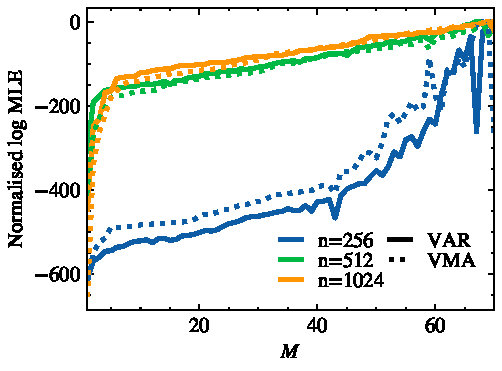
\includegraphics[width=\columnwidth]{sim_basis.pdf}
  \caption{The relationship between the number of basis functions and the maximum likelihood estimate for both VAR2 and VMA1 models with different lengths. \avi{remake plot using $L_2$ instead of $L2$. Also speciofy the difference between a) and b) }}
  \label{fig:sim_basis}
\end{figure}

Figure~\ref{fig:sim_error_violins} panels (ab) displays the $L_2$ errors (see Appendix~\ref{appdx:simstudy}) from both the SGVB and VNPC methods, computed using the true spectral densities of the (a) VAR(2) simulations and (b) VMA(1) simulations. 
Figure~\ref{fig:sim_error_violins}(c) displays the speed-up factor of the SGVB compared to the VNPC method. 
As the sample size increases, both methods obtain lower (and similar) $L_2$ errors, while the speed-up factor for SGVB increases to more than 50 times VNPC.

While the accuracy of \ac{SGVB} is only slightly lower than that of VNPC, the computation time is reduced by a factor of about 50 when $n=1024$.
Furthermore, the simulation study provides empirical evidence that the \ac{SGVB} approach is consistent, i.e., with increasing sample size, the posterior distributions concentrate around the true spectral density ($L_2$ error are $<0.3$). 

\begin{figure}
  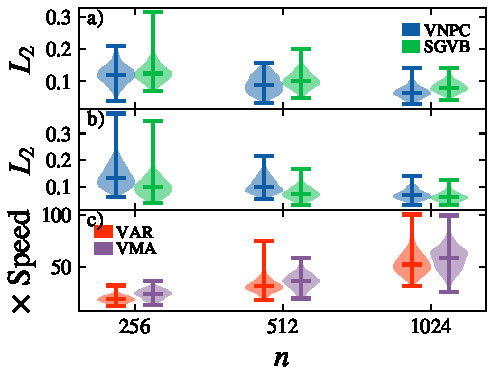
\includegraphics[width=\columnwidth]{sim_error_violins.pdf}
  \caption{Violin plots of 500 $L_2$ errors obtained from applying the VNPC and \ac{SGVB} methods to 500 realizations of (a) the VAR(2) model and (b) the VMA(1) model with different sample sizes. (c) displays the speed-up factor, defined as the ratio of the time taken by the VNPC method to that taken by the \ac{SGVB} method for different models and sample sizes.}
  \label{fig:sim_error_violins}
\end{figure}
 
Refer to Appendix~\ref{appdx:simstudy} for more details on the results of the simulation study. 




\section{Application to ET noise}
\label{sec:application}
\subsection{Data Generation}
\label{sec:data_gen}

We use 2000 seconds of  Gaussian noise colored with the design sensitivity of the xylophone configuration of the ET sampled at 2048 Hz which yields a time series of length 4,096K.  
\footnote{Please note that the sensitivity curve used here is the previously called `ET-D' sensitivity curve. We choose tho use this curve rather than the slightly updated version presented in \cite{Branchesi:2023mws}, to compare more directly to previous work \cite{Janssens2023}. The small difference between PSD curves will have no impact on the key conclusions of the applicability of the work presented in this paper.}~\cite{Hild_2009,Hild:2010id}. 
In the rest of the
paper we refer to this colored Gaussian noise as `ET noise' 

%\RM{What is the psd formula?} %\KJ{There is no straightforward formula. It is a complex combination from a handful key and another dozen smaller noise sources.}
% Note that despite the fact that
%we use identical noise, the X, Y and Z data are dierent
%Gaussian noise realisations.
To simulate  non-identical correlated noise in the X, Y and Z channels, following \cite{Janssens2023}, we additionally injected another set of colored Gaussian noise, now with the shape of Gaussian peaks in the frequency domain. The Gaussian peaks are defined by the PSD
\begin{equation}
    S_n^{\mathrm{GP}}(f)= \left( \frac{A}{\sqrt{2\pi}}\exp\left\{ 
- \frac{(f-\mu)^2}{2\sigma^2}\right\}\right)^2\ ,
\end{equation}
with amplitude $A$, frequency peak location $\mu$ and spread $\sigma$.
Gaussian noise was injected in the X channel at $10$ Hz and 50 Hz, at 10
Hz and 90 Hz in the Y channel and at 50 Hz and 90 Hz in the Z channel with respective amplitudes at 10, 50 and 90 Hz of $4\times 10^{-24}$, $2\times 10^{-24}$ and $1.5\times 10^{-24}$ and $\sigma=1$ for all frequencies. Identical data was used for the Gaussian peaks at the same frequencies as to induce correlated noise between each pair of channels.
Whereas we recognize this dataset to be unrealistic in its simplicity and high level of separability due to the highly unique nature of the correlated noise terms (i.e. the Gaussian peaks), we believe it to be a good data set for initial demonstrations. Afterwards the goal is to increase complexity and approach a more realistic noise scenario such as the inclusion of correlated magnetic and/or Newtonian noise.



\subsection{Data Analysis}

% Introduce the cases clearly. 
% Maybe introduce this in the datageneration section.
% \noindent
% Case 1: correlated data - coherence \\
% Case 2: uncorrelated data - coherence \\
% Case 3: uncorrelated data - coherence = 0

% \begin{itemize}
%   \item Analysis of ET noise with coherently injected Gaussian peaks.
%   \item Analysis of ET noise with incoherently injected Gaussian peaks.
%   \begin{itemize}
%       \item with the original \ac{SGVB} method estimating the co-spectra
%       \item with the modified \ac{SGVB} method (off-diagonals not estimated) 
%   \end{itemize}
% \end{itemize}

We conduct three analyses:
\begin{enumerate}[label=Case \arabic*:] 
    \item Analysis on ET noise with correlated noise as described in Section~\ref{sec:data_gen},
    \item Analysis on ET noise (no correlated noise), 
    \item Analysis on ET noise (no correlated noise) assuming there are no-cross diagonal elements of the multivariate PSD \avi{We need to reword this..}
\end{enumerate}
\todo{the 'case' is going into the margin}

The dataset of each case of the ET noise can be considered as a three dimensional Gaussian stationary multivariate time series of length 4,096K. 
To handle such a large data set, in this application, the whole dataset is evenly divided into 125 segments each of length 32,738.
The Fourier-transformed version of each segment serves as input data for a blocked Whittle likelihood. 
Every Whittle likelihood block with corresponding input segment has the same basis function expressions for spectral density matrix. 
Since the Fourier transform is an even function, the number of frequency points for each segment is now 16384. 
Consequently, the product of 125 Whittle likelihood blocks forms a new Whittle likelihood representing  the entire dataset. 
In all three cases, since Gaussian peaks are injected at the first 128 Hz, we can only extract the corresponding data from each segment that after the Fourier transform as the input dataset for each Whittle likelihood block, this can improve the computational efficiency.

In order to optimize the number of basis functions in the \ac{SGVB} method for three cases, the effect of the number of basis functions on the maximum log Whittle likelihood is observed. Figure~\ref{et_corr_basis_funs_vs_mle} illustrates the relationship between the number of basis functions and the corresponding maximized log Whittle likelihood values. During the maximization process, the learning rate for gradient ascent is set to 0.002, and the number of iterations is set to 10,000, with the number of basis functions ranging from 100 to 700 in increments of 10. Based on the Figure~\ref{et_corr_basis_funs_vs_mle}, the optimal number of basis functions for three cases can be set to 450. Python function \hyperopt is used to optimise the learning rate $\tau_1$ from the first step to maximise the ELBO, the range is set from 0.002 to 0.02 and the maximum number of evaluations is set to 10, the $\tau_2$ from the second step is set to 0.05.
\begin{figure}
\centering
  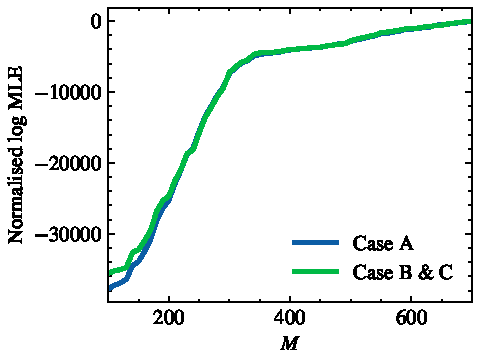
\includegraphics[width=\columnwidth]{et_basis_fns.pdf}
  \caption{The relationship between the number of basis functions and the maximum likelihood estimate for three cases. \avi{Set xlim to be the first and last M}}
  \label{et_corr_basis_funs_vs_mle}
\end{figure}

\avi{show matrix PSD plots here}



\avi{After we talk about the PSD, discuss the coherences}


In this application, the squared coherence is used to investigate the correlation between any two channels. If the value of squared coherence $C_{xy}(f_k)$ is closer to 1, this means the two channels have a strong association at frequency $f_k$. If it is closer to 0, this indicates the association at the corresponding frequency is very weak between the two channels. Recall that the squared coherence $C_{xy}(f_k)$ between two components of a multivariate time series for frequency $f_k$ is defined as:
\begin{align}\label{squared coh}
C_{xy}(f_k) = \frac{|\S_{xy}(f_k)|^2}{\S_{xx}(f_k)\S_{yy}(f_k)}
\end{align}
where $\S_{xy}(f_k)$ for $x,y = 1,2,...,p$ and $x\neq y$ represents the cross-spectral density between components $x$ and $y$ at frequency $f_k$, while $\S_{ii}(\nu_k)$ and $\S_{jj}(\nu_k)$ represent the spectral densities of components $x$ and $y$, respectively, at frequency $f_k$.


The following plots (Figures \ref{fig:test} and \ref{caseAB_coh}) show the estimated power spectral densities and the squared coherences for three cases given the optimised learning rate and the corresponding parameters under the maximised ELBO.
\begin{figure*}[h]
\centering
\begin{subfigure}{\columnwidth}
  \centering
  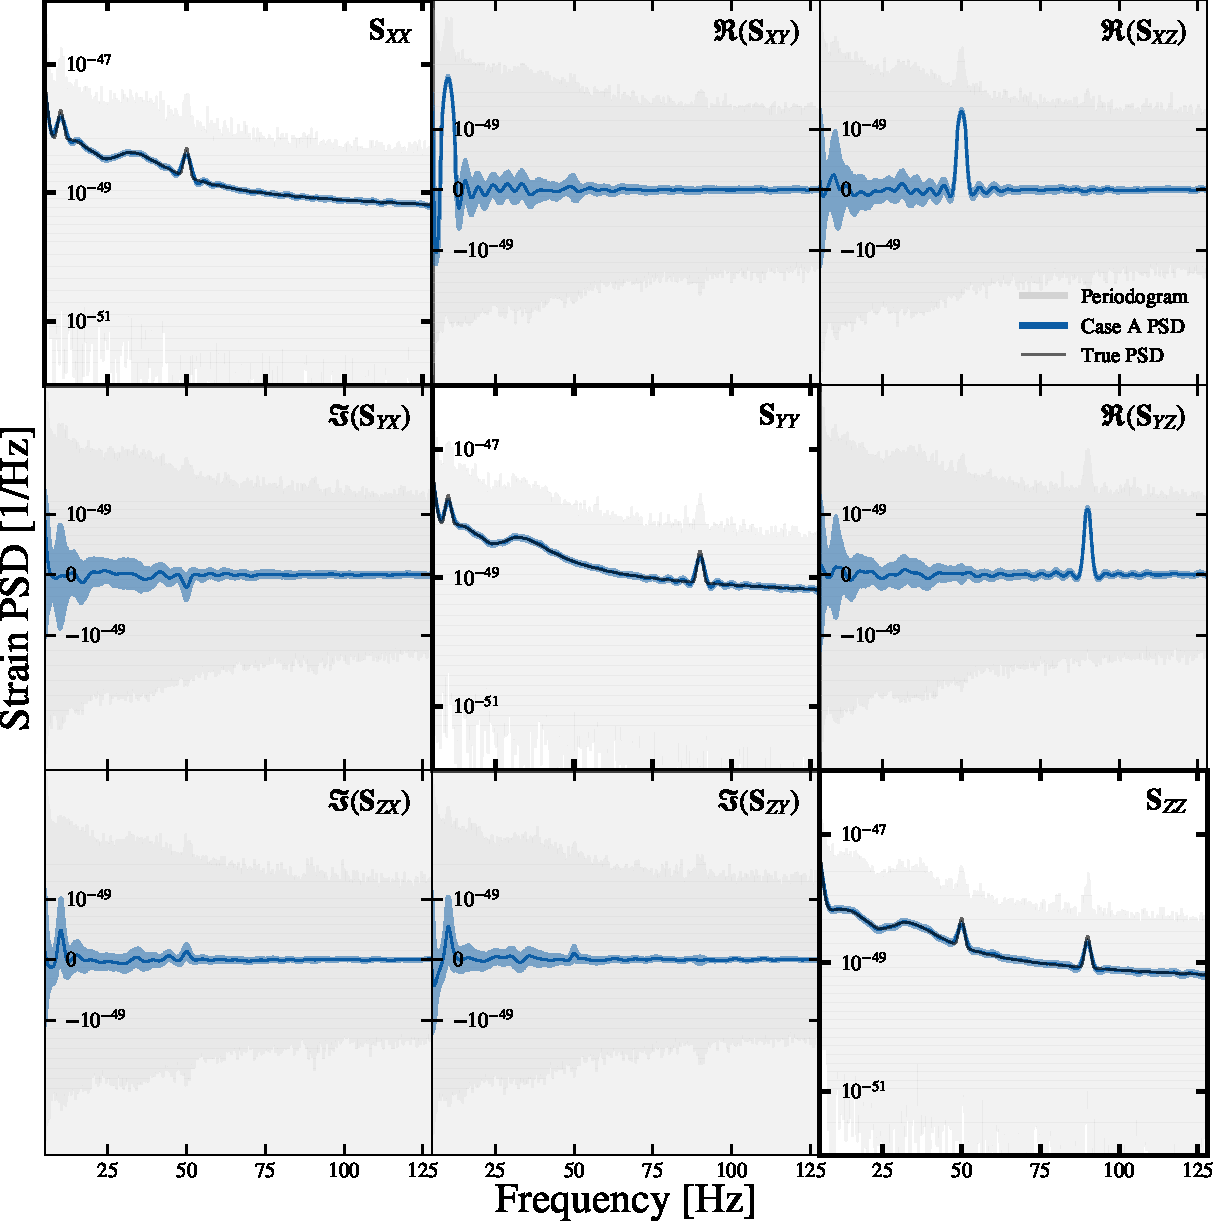
\includegraphics[width=1.05\columnwidth]{caseA_psd.pdf}
  \caption{Case A PSD}
  \label{fig:caseA_psd}
\end{subfigure}
\hfill
\begin{subfigure}{\columnwidth}
  \centering
  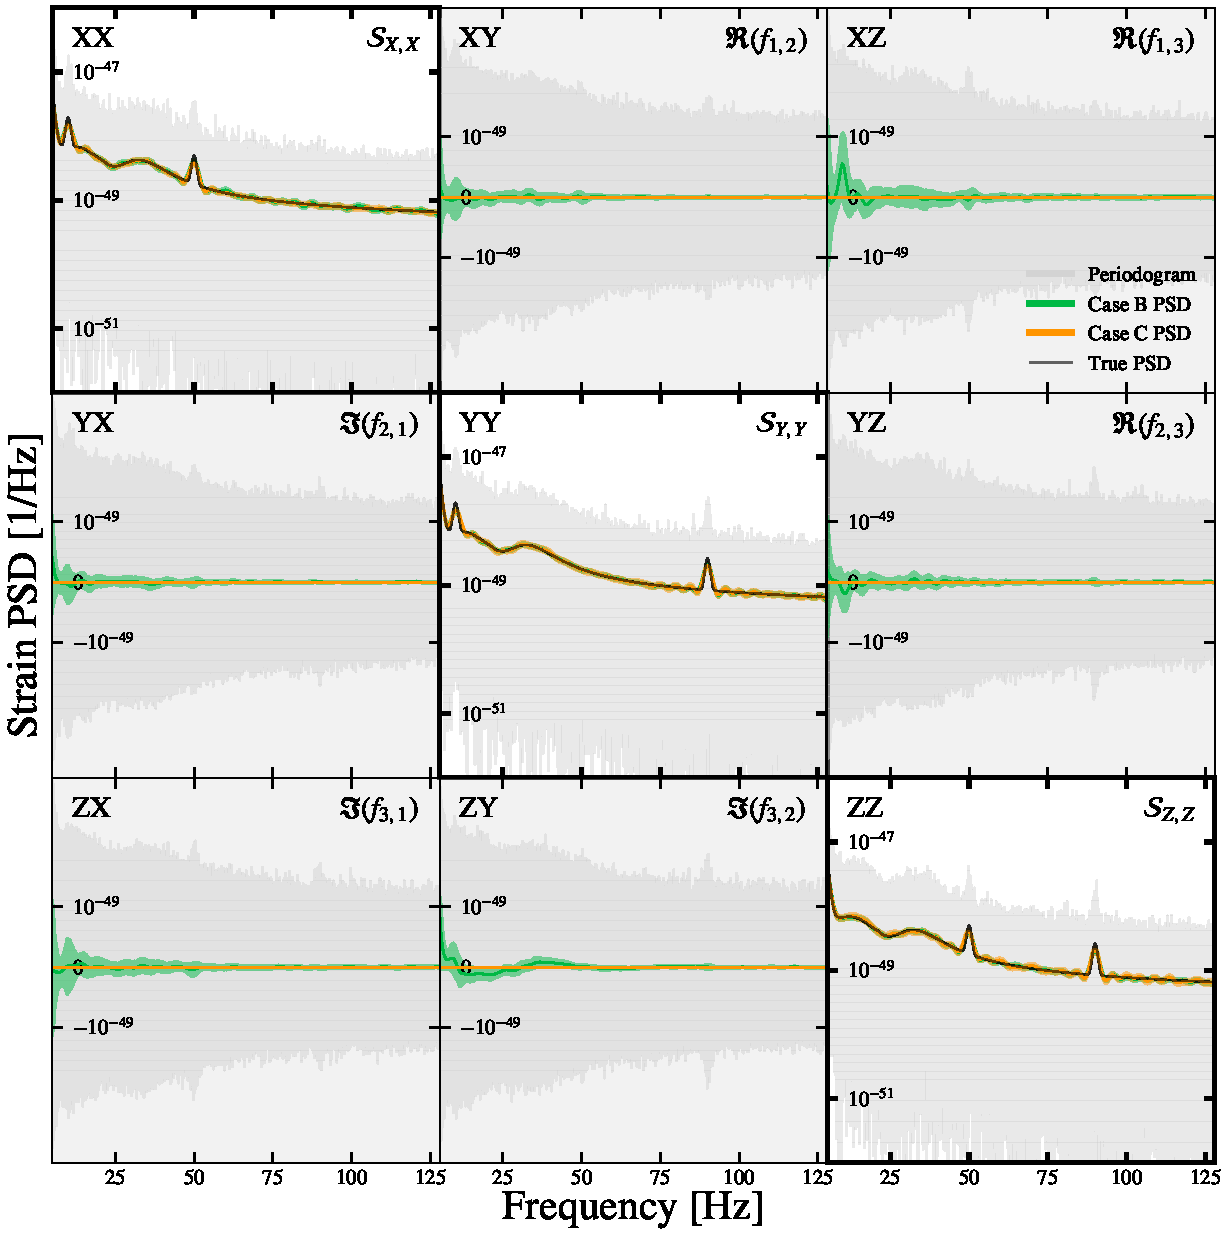
\includegraphics[width=1.05\columnwidth]{caseBC_psd.pdf}
  \caption{Case B and C PSD}
  \label{fig:caseBC_psd}
\end{subfigure}
\caption{Spectral density estimates for three cases of ET noise data. Estimates are shown for VI (SGVB, green with 90\% CI) and periodogram (grey).}
\label{fig:test}
\end{figure*}

\begin{figure}
  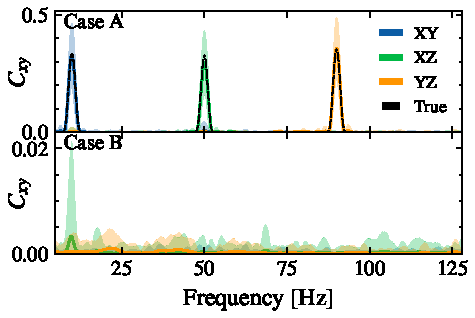
\includegraphics[width=\columnwidth]{caseAB_coh.pdf}
  \caption{Squared coherence estimates for differenct cases of ET noise data.}
  \label{caseAB_coh}
\end{figure}







\section{Discussion}


Take a look at yixuan's sec 5.3 and conclusions 


% Note that for the VAR2 model, VNPC consistently demonstrates higher accuracy across all data lengths, 
% Therefore, while VNPC may be more accurate but computationally costly, \ac{SGVB} presents an attractive alternative, especially for larger datasets or when rapid computation is necessary.

% Show ET results, compare MCMC and \ac{SGVB} on simulated ET noise with injected Gaussian peaks

% \avi{Even if we can run the MCMC, comment on how long MCMC might take (estimate based on time for one LNL evaluation)}

% \begin{itemize}
%     \item VI Results, data with no correlation 
%     \item VI Results, data with correlation
%     \item VI no-off diagnals, data with correlation 
% \end{itemize}



In this study, the \ac{SGVB} method is utilized to estimate the spectral densities for three cases of simulated ET noise data, and construct the corresponding squared coherences for every pair of channels to obtain the correlation between them in the certain frequencies. For all of the three cases, it is evident that in the X channel, prominent peaks are observed at 10 Hz and 50 Hz. Similarly, for the Y channel, peaks are observed at 10 Hz and 90 Hz, while for the Z channel, peaks are observed at 50 Hz and 90 Hz. For case A, it is evident that there is significant coherence between channels X and Y at 10 Hz, between channels X and Z at 50 Hz, and between channels Y and Z at 90 Hz. For case B, although the ET noise data with uncorrelated noise is analysed, small fluctuations can still be observed in the off-diagonal subplots represent the real and imaginary part of the estimated spectral densities. The small correlations can also be observed from the  corresponding squared coherences. For case C, by treating the cross spectrum as zero, the estimated spectral densities for three channels are independent, this results in the square coherence is 0 as well.


% \begin{itemize}
%     \item demonstrated nonparametric methods to estimate correlated noise in ET (or LISA) data that can handle long time series 
%     \item in future: simultaneous estimation of SGWB and noise
%     \item hyperparameter optimization, adaptive learning rates
% \end{itemize}



During the \ac{ET} era, managing correlated noise will be essential for maximising \ac{ET} scientific capabilities~\cite{Cireddu:2023:arXiv}.
We demonstrate a VI method for estimating a multivariate PSD for a \ac{GW} interferometer network under the influence of correlated noise and demonstrate how to quantify coherence. 
We demonstrate how the coherence changes as the noise correlation is adjusted. 
Future efforts will evaluate the impact of \ac{PE} for a compact-binary coalescence \ac{GW} signal in correlated noise, using a multivariate PSD and independent PSDs. 
Additional work will explore the automation of hyper-parameter optimisation to tune the \ac{VI} parameters. 


\begin{acknowledgments}
We like to thank Zhixiong Hu and Racquel Prado for making their code publicly available and for helpful discussions. NC, JEL, PMR, RM, and AV gratefully acknowledge support  by the Marsden Fund Council grant MFP-UOA2131 from New Zealand Government funding, managed by the Royal Society Te Apārangi. We thank the New Zealand eScience Infrastructure
(NeSI) \url{https://www.nesi.org.nz} for the use of their high performance computing facilities and
the Centre for eResearch at the University of Auckland for their technical
support.
\end{acknowledgments}
\bibliography{reference}

\appendix  


\section{Accuracy of the blocked  Whittle likelihood}
\label{appdx:blocked_lnl}
\begin{figure}[h]
  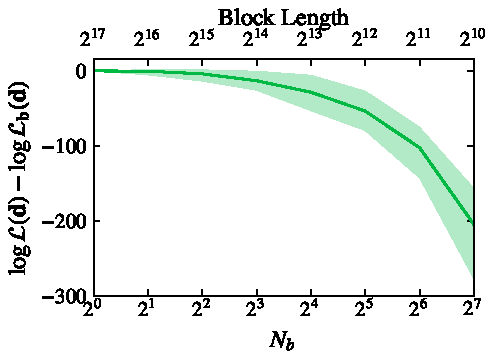
\includegraphics[width=\columnwidth]{lnl_vs_nchunks}
  \caption{Blocked Whittle likelihood as a function of the number of blocks utilised.}
  \label{lnl_vs_nchunks}
\end{figure}
\todo{not chunk -- block}





\section{Simulation study details}




\label{appdx:simstudy}
% The VAR(2) model is defined by
% \begin{align}
% Z_t = \begin{pmatrix}0.5 & 0 \\0 & -0.3\end{pmatrix}\underline{Z}_{t-1}+\begin{pmatrix}0 & 0 \\0 & -0.5\end{pmatrix}\underline{Z}_{t-2}+\underline{e}_t, %\quad \underline{e}_t\overset{iid}{\sim}N \left(\bm{0}, \begin{pmatrix}1 & 0.9 \\0.9 & 1\end{pmatrix} \right)
% \end{align}
%  where $\underline{e}_t\overset{iid}{\sim}N \left(\bm{0}, \begin{pmatrix}1 & 0.9 \\0.9 & 1 \end{pmatrix}  \right) $ and the VMA(1) is given by
% \begin{align}
% \underline{Z}_t =\underline{e}_t+\begin{pmatrix}-0.75 & 0.5 \\0.5 & 0.75\end{pmatrix}\underline{e}_{t-1}, \quad \underline{e}_t\overset{iid}{\sim}N \left(\bm{0}, \begin{pmatrix}1 & 0.5 \\0.5 & 1\end{pmatrix}\right)\ .
% \end{align}


Let $\hat{\bm{f}}$ denotes the estimated spectral density matrix for one realization, and let $\bm{f}_0$ be the true spectral density matrix. 
The $L_2$ error is defined as
\begin{eqnarray*}
||\hat{\bm{f}} - \bm{f}_0||_{L_2} &=& \left(\int_{0}^{0.5} ||\hat{\bm{f}}_0(\nu) - \bm{f}_0||^2 d\nu \right)^{\frac{1}{2}} \\
&\approx &\left(\frac{1}{N} \sum_{k=1}^{N}||\hat{\bm{f}}_0(\nu_k)-\bm{f}_0(\nu_k)||^2 \right)^{\frac{1}{2}}
\end{eqnarray*}
where $\Vert \cdot \Vert$ denotes the Frobenius norm, i.e., defined for a complex $p\times p$ matrix $\A$ by
$\displaystyle \Vert \A\Vert= \sqrt{\sum_{i,j} |a_{ij}|^2}$.

The following two tables present the average  $L_2$ errors, empirical coverage and median width of pointwise 90\% credible regions as well as the average computation time per realization (in seconds), for the 500 realizations of both models with different lengths using the VNPC and \ac{SGVB} methods. \hyperref[table l1l2 var2]{Table 1} gives the results for  the VAR(2) model, while the \hyperref[table l1l2 vma1]{Table 2} displays those for  the VMA(1) model.


\begingroup
\renewcommand{\arraystretch}{1.4} 
\begin{table}[h]
\centering
\begin{tabular}{ccccccc}
\hline
\multicolumn{7}{c}{VAR(2) model} \\
\quad & \multicolumn{2}{c}{$n=256$}  & \multicolumn{2}{c}{$n = 512$}  & \multicolumn{2}{c}{$n = 1024$}\\
\hline
\quad & {VNPC} & {SGVB} & {VNPC} & {SGVB} & {VNPC} & {SGVB}\\
%{$L_1$ error} & 0.098 & 0.133 & 0.078 & 0.073 & 0.061 & 0.049\\
{$L_2$ error} & 0.129 & 0.121 & 0.103 & 0.091 & 0.082 & 0.066\\
{Coverage} & 0.860 & 0.614 & 0.845 & 0.658 & 0.832 & 0.663\\
{Width $f_{11}$} & 0.085 & 0.058 & 0.060 & 0.043 & 0.044 & 0.031\\
{Width $\Re f_{12}$} & 0.091 & 0.056 & 0.067 & 0.042 & 0.050 & 0.031\\
{Width $\Im f_{21}$} & 0.074 & 0.045 & 0.056 & 0.039 & 0.042 & 0.028\\
{Width $f_{22}$} & 0.132 & 0.072 & 0.092 & 0.053 & 0.067& 0.036\\
{Time} & 5{\rm K} & 300 & 10{\rm K} & 300 & 19{\rm K} & 350\\
\hline
\end{tabular}
\caption{{\small Comparison of average  $L_2$ errors, empirical coverage and median width of pointwise 90\%
credible regions along with the average computation time (in seconds), for 500 realizations using VNPC and \ac{SGVB} methods across different sample sizes ($n=256$, $512$, and $1024$) for the VAR(2) model.}}
\label{table l1l2 var2} 
\end{table}


\begin{table}[h]
\centering
\begin{tabular}{ccccccc}
\hline
\multicolumn{7}{c}{VMA(1) model}\\
\quad & \multicolumn{2}{c}{$n=256$}  & \multicolumn{2}{c}{$n = 512$}  & \multicolumn{2}{c}{$n = 1024$}\\
\hline
\quad & {VNPC} & {SGVB} & {VNPC} & {SGVB} & {VNPC} & {SGVB}\\
%{$L_1$ error} & 0.081 & 0.141 & 0.059 & 0.092 & 0.048 & 0.059\\
{$L_2$ error} & 0.101 & 0.138 & 0.075 & 0.106 & 0.061 & 0.069\\
{Coverage} & 0.905 & 0.638 & 0.893 & 0.620 & 0.840 & 0.662\\
{Width $f_{11}$} & 0.118 & 0.086 & 0.081 & 0.070 & 0.058 & 0.053\\
{Width $\Re f_{12}$} & 0.077 & 0.062 & 0.054 & 0.042 & 0.038 & 0.029\\
{Width $\Im f_{21}$} & 0.063 & 0.044 & 0.041 & 0.032 & 0.029 & 0.026\\
{Width $f_{22}$} & 0.173 & 0.180 & 0.122 & 0.126 & 0.084 & 0.097\\
{Time [s]} & 4{\rm K} & 200 & 7{\rm K} & 200 & 12{\rm K} & 200 \hspace{-.5em} \\
\hline
\end{tabular}
\caption{{\small Comparison of average $L_2$ errors, empirical coverage and median width of pointwise 90\%
credible regions along with the average computation time (in seconds), for 500 realizations using VNPC and \ac{SGVB} methods across different sample sizes ($n=256$, $512$, and $1024$) for the VMA(1) model.}}
\label{table l1l2 vma1} 
\end{table}
\endgroup

% From the tabular comparison, \ac{SGVB} generates a narrower confidence interval than VNPC. This phenomenon can be attributed to the tendency of variational inference methods to underestimate the marginal variances of the target distribution during the optimization process. This process is equivalent to minimising $KL(q||p)$, where $q$ is the surrogate distribution and $p$ is the target posterior distribution. During this optimization, when $q$ assigns more probability mass to regions where $p$ has less probability mass, the KL divergence becomes very large. To avoid this, the optimization process leads the surrogate distribution to focus on high probability regions of the true posterior \cite{Blei2017}. \ac{SGVB} is a method developed based on mean-field variational inference, and assumes that the posterior distribution can be decomposed into independent factors. However, in practice, parameters are often correlated, especially in complex models. This assumption leads to ignoring the correlations between parameters, resulting in an underestimation of overall uncertainty \cite{Blei2006}. Furthermore, the compactness property of \ac{SGVB} constrains $q$ to a fixed-shape distribution family (multivariate Gaussian distribution). The optimization process can only adjust the mean and covariance of this distribution but cannot alter its fundamental shape. This limitation may lead to underestimation of probability mass in certain regions of the true posterior, thus underestimating the overall uncertainty \cite{Turner2011}. \cite{Wang2005} provided that the covariance matrix obtained by the variational Bayesian method differs from the inverse of the Fisher information matrix by a nonnegative definite matrix. This result demonstrates that the covariance matrix obtained by the variational Bayesian method is typically smaller, implying that credible interval estimations based on the variational Bayesian method are usually narrower than those based on the true posterior distribution.





\end{document}
%
% ****** End of file apssamp.tex ******
